\section{Source Code Overview}
This section is intended to help you familiarize with the SimComp codebase. Since both UIs are dependent on the Simulator API it is crucial that you're familiar with it before you start this section. Figure \ref{fig:relation} shows the relation between the different parts of the SimComp project.

\begin{figure}[H]
\centering
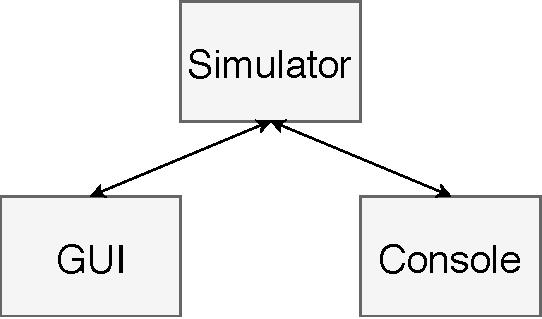
\includegraphics[scale=0.8]{img/SimComp-relation.pdf}
\caption{SimComp project relation}
\label{fig:relation}
\end{figure}

\subsection{Simulator}
\subsubsection{File Description}
\begin{description}
\item[isa.h/.cpp] - Contains the \texttt{Isa} class that defines the instruction set and functions that help interpreting and printing instructions.

\item[loader.h/.cpp] - Contains the \texttt{Loader} class that reads the sasm-format and generates instructions that are written to the instructions memory.

\item[logger.h/.cpp] - Contains the \texttt{Logger} class used to log simulator execution. 

\item[memory.h/.cpp] - Contains the \texttt{Memory} class used by the \texttt{ComputerSimulation} class to store data- and instruction memory. 

\item[program.h/.cpp] - Contains the \texttt{Program} struct that stores information about a assembler program, the struct is needed by \texttt{ComuputerSimulation} to generate instructions.

\item[compSim.h/.cpp] - Contains the \texttt{ComputerSimulation} class that is responsible for control and execution of simulation. The class is designed to be the access point for the API. 
\end{description}

\subsection{Console}
\subsubsection{File Description}
\begin{description}
\item[main.cpp] - Entry point that uses the first argument as the path to construct an instance of \texttt{ConsoleUi}. 

\item[consoleUI.h/.cpp] - Contains the class \texttt{ConsoleUi} which creates and controls a console user interface. \texttt{ConsoleUi} is also responsible for creating an instance of \texttt{ComputerSimulation}.
\item[config.h/.cpp] - Contains functions for finding assembler programs in a folder.
\item[utils.h/.cpp] - Contains utility functions for creating a console ui.
\end{description}

\subsection{GUI}
\subsubsection{File Description}
\begin{description}
\item[main.cpp] - Entry point. Starts application and creates an instance of \texttt{MainWindow}. 

\item [mainwindow.h/.cpp] - The \texttt{MainWindow} class inherits \texttt{QMainWindow}. It is responsible for creating and controlling all dock windows, the menubar, statusbar, styling and the central widget. The central widget is a \texttt{QTabWidget} populated with one instance of \texttt{RunWidget} and one of \texttt{IdeWidget}. Figure \ref{fig:qmainwindowlayout} shows how these are organized. For more information on \texttt{QMainWindow} see [\ref{qmainwindow}].

\begin{figure}[H]
\centering
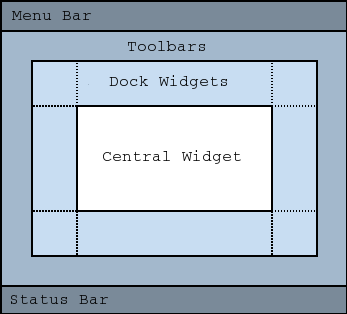
\includegraphics[scale=0.5]{img/mainwindowlayout.png}
\caption{QMainWindow layout \cite{qt}}
\label{fig:qmainwindowlayout}
\end{figure}


\item [runwidget.h/.cpp] - Contains the \texttt{RunWidget} and the \texttt{SimulatorThread} classes. \\ \\ \texttt{RunWidget} inherits \texttt{QWidget} and is responsible for simulator execution. Graphically, the widget consists of the execution table which show information relevant to execution, see figure \ref{fig:runwidget}. \texttt{RunWidget} is one of the two tabs in the \texttt{QTabWidget} set as central widget by \texttt{MainWindow}. \\ \\
\texttt{SimulatorThread} inherits \texttt{QThread}. The class overrides the \texttt{virtual void QThread::run()} function to start the simulator by invoking \texttt{void ComputerSimulation::run()}. Calling \texttt{SimulatorThread::run()} will therefore start the simulator in RUN-mode in a thread. The class is constructed with a pointer to a \texttt{ComputerSimulation} instance.

\begin{figure}[H]
\centering
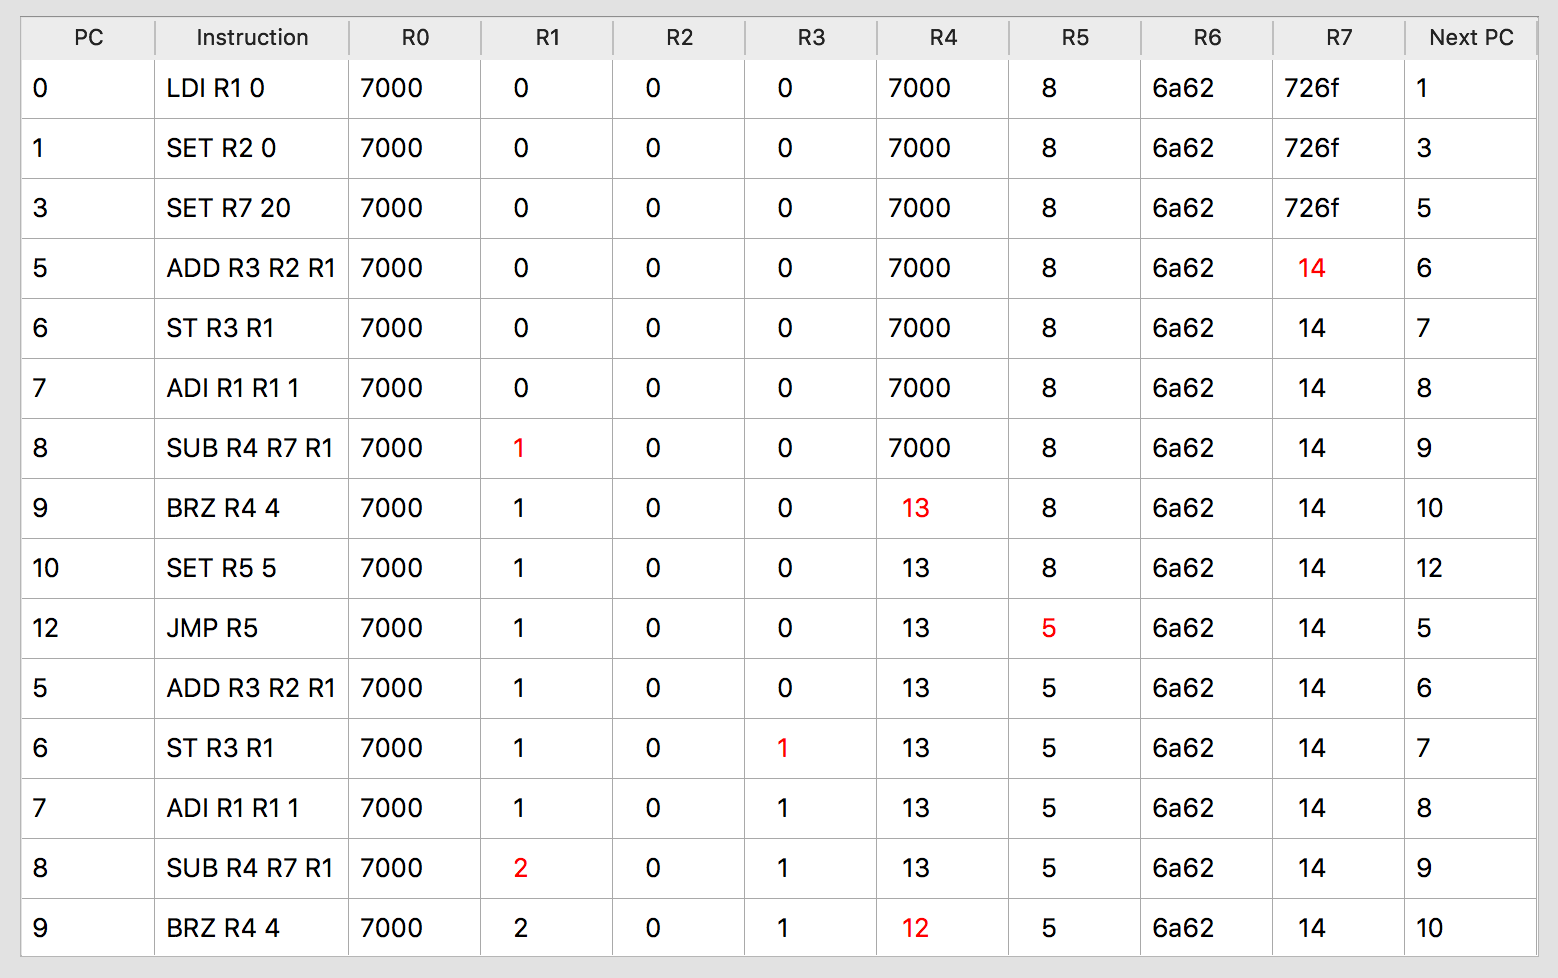
\includegraphics[scale=0.3]{img/RunWidget.png}
\caption{Screenshot of a RunWidget used in the SimComp GUI.}
\label{fig:runwidget}
\end{figure}


\item [idewidget.h/.cpp] - The \texttt{IdeWidget} class inherits \texttt{QPlainTextEdit} and acts as a standalone ide widget. Graphically, the widgets consists of the editing area and a left sidebar with line numbers and breakpoints, see figure \ref{fig:idewidget}. The class is responsible for creating, editing, opening and saving assembler programs. \texttt{IdeWidget} is the second of the two tabs in the \texttt{QTabWidget} set as central widget by \texttt{MainWindow}.

\begin{figure}[H]
\centering
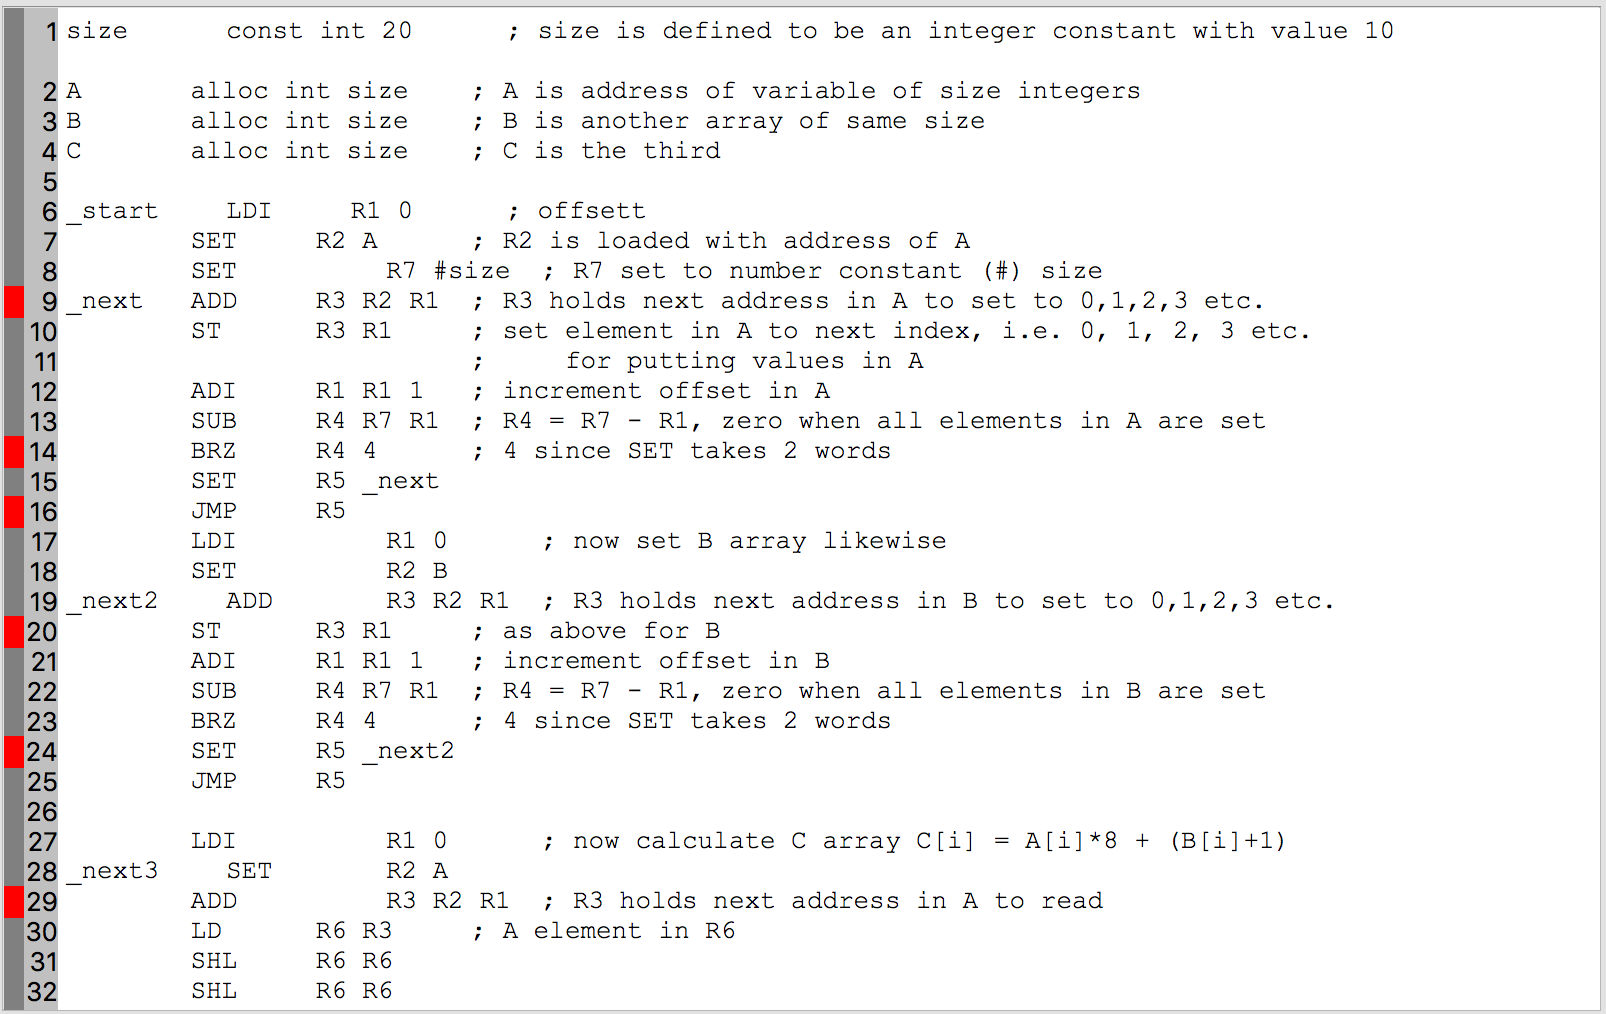
\includegraphics[scale=0.3]{img/IdeWidget.png}
\caption{Screenshot a IdeWidget used in the SimComp GUI.}
\label{fig:idewidget}
\end{figure}

\item [memorywindow.h/.cpp] - The \texttt{MemoryWindow} class inherits \texttt{QWidget} and is should be used as a top-level window. The window is used to display memory areas, see fig \ref{fig:memorywindow}. A \texttt{QSplitter} is used to fill the top layout of the window. The splitter is populated by two widgets: 

\begin{itemize}
    \item The left side is a \texttt{QTabWidget} that contains two tabs, one with a table- (\texttt{QTableWidget}) and one with an graphical (\texttt{MemoryMap}) representation of the memory area.
    \item The rigth side is a \texttt{QWidget} which is used as a container for the configuration portion of the \texttt{MemoryWindow}.
\end{itemize}

\begin{figure}[H]
\centering
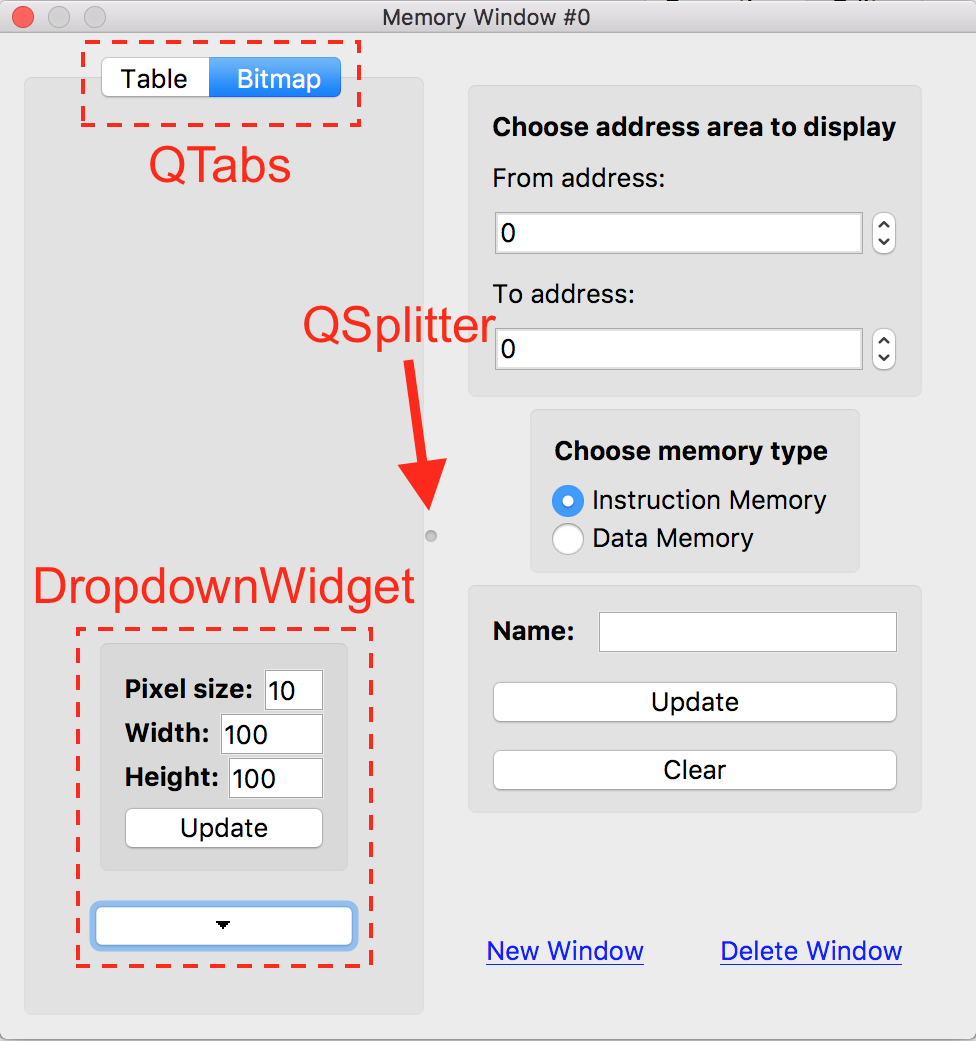
\includegraphics[scale=0.35]{img/MemoryWindow.png}
\caption{Screenshot of a MemoryWindow used in SimComp GUI.}
\label{fig:memorywindow}
\end{figure}

\item [memorymap.h/.cpp] - The \texttt{MemoryMap} class inherits \texttt{QWidget} and overrides the \texttt{virtual void QWidget::paintEvent(QPaintEvent *event)} function to paint it self as a bitmap with the values set in the member variable \texttt{hexMap}. The \texttt{hexMap} is a \texttt{std::vector<std::string>} and is set using the \texttt{setVector} member function.

\item [dropdownwidget.h/.cpp] - The \texttt{DropDownWidget} class inherits \texttt{QWidget}. It acts as a drop-down menu that can be populated with widgets using the \texttt{addWidget} function.

\item [fileviewer.h/.cpp] - The \texttt{FileViewer} class inherits \texttt{QWidget} and is responsible for displaying file information, see figure \ref{fig:fileviewer}. It also provides an additional way to choose assembler program. 

\begin{figure}[H]
\centering
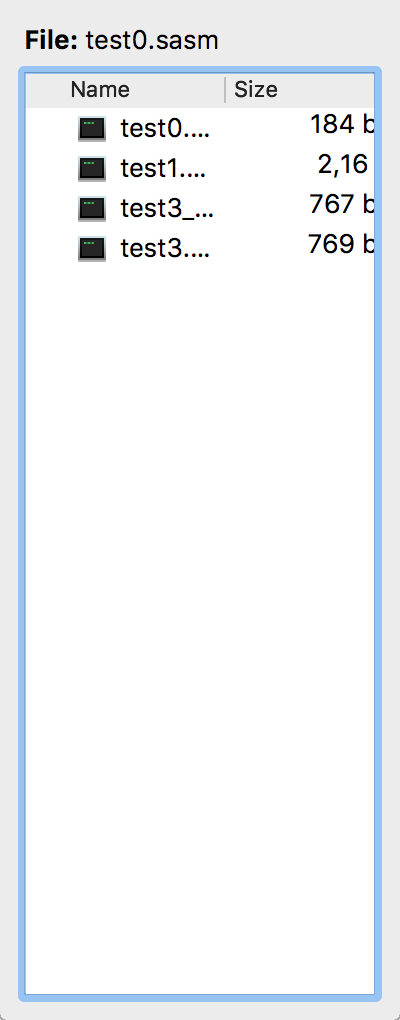
\includegraphics[scale=0.3]{img/FileViewer.png}
\caption{Screenshot of a FileViewer used in the SimComp GUI.}
\label{fig:fileviewer}
\end{figure}

\item [performancechart.h/.cpp] - The \texttt{PerformanceChart} inherits \texttt{QChart} and is used to display a live plot of the simulator performance (MIPS), see figure \ref{fig:performancechart}.

\begin{figure}[H]
\centering
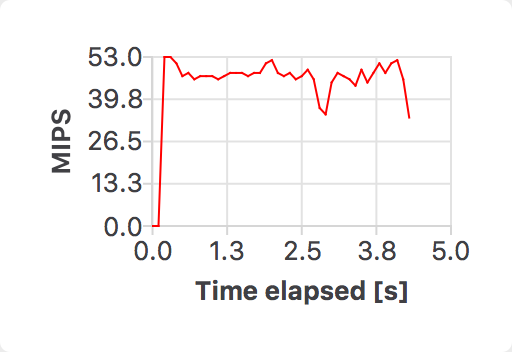
\includegraphics[scale=0.6]{img/PerformanceChart.png}
\caption{Screenshot of a PerformanceChart used in the SimComp GUI.}
\label{fig:performancechart}
\end{figure}

\item [globals.h] - Used to store global constants in the \texttt{globals} namespace.

\end{description}

\subsubsection{Important connections}
Qt Object Communication relies on sending and receiving signals. The receiver responds to a signal by calling a function (slot). The most important of these signal-slot connections are listed in table \ref{table:connections}. \textbf{Note} that Lambda* denotes C++11 lambda functions that are not members, therefore there is no receiver.
\begin{table}[!ht]
\caption{Important Qt connections in the SimComp GUI project.}
\makebox[\linewidth]{
\begin{tabular}{|l|l|l|l|}
\hline
\rowcolor[HTML]{C0C0C0} 
\textbf{Sender} & \textbf{Signal}                                     & \textbf{Receiver} & \textbf{Slot/Function}                                                                       \\ \hline
RunWidget       & instructionCountChanged(int) & Lambda*           & \begin{tabular}[c]{@{}l@{}}Updates status bar with\\ the new instruction count.\end{tabular} \\ \hline
RunWidget       & performanceChanged(double)               & PerformanceChart  & updatePerformance(double)                                                               \\ \hline
IdeWidget       & fileChanged(QString)                 & RunWidget         & load(QString)                                                                       \\ \hline
IdeWidget       & fileChanged(QString)                 & Lambda*           & Set FileViewer to filename.                                                                  \\ \hline
IdeWidget       & breakPointsChanged()                                & Lambda*           & \begin{tabular}[c]{@{}l@{}}Sets breakpoints in \\ RunWidget.\end{tabular}                    \\ \hline
FileViewer      & changeFile(QString)                  & IdeWidget         & open(QString)                                                                       \\ \hline
SimulatorThread & finished()                                          & RunWidget         & runFinished()                                                                                \\ \hline
QTimer          & timeout()                                           & RunWidget         & updatePerformance()                                                                          \\ \hline
\end{tabular}
}
\label{table:connections}
\end{table}
